% ============================================================
%  template.tex —— 主文件，只写内容
%  编译方式：XeLaTeX（支持中文），编译两次生成目录
% ============================================================
\documentclass[notheorems]{beamer}

\input{pptheader.tex}
\input{mycommand.tex}

\begin{document}
	
	% ============================================================
	%  元信息：修改标题、作者、单位、日期
	% ============================================================
	\title[科研汇报与片段教学]{科研工作汇报与片段教学展示}
	\subtitle{%
		\vspace{4pt}
		{\small\textbf{科研汇报：}基于高阶有限元的变密度拓扑优化} \\[6pt]
		{\small\textbf{片段教学：}函数极限的夹逼性定理}
	}
	
	% 在 [] 中填入短作者名，避免把导师信息和排版命令也带入页脚
	\author[何亮]{报告人：何亮 \\
		\vspace{5pt}
		导师：{\CJKfontspec{SimSun}魏华祎} 教授}
	
	% [] 中填入单位简称
	\institute[湘大数学院]{
		\vspace{5pt}
		湘潭大学 \\
		数学与计算科学学院
	}
	\date{\today}
	
	% ---- 封面页 ----
	\frame[plain]{\titlepage}
	
	% ---- 每节开始自动插入目录页 ----
	\AtBeginSection[]{
		\frame<beamer>{
			\frametitle{目录}
			\tableofcontents[currentsection]
		}
	}
	
	% ---- 全局目录（可选） ----
	\begin{frame}
		\frametitle{目录}
		\tableofcontents
	\end{frame}
	
	
	% ============================================================
	\section{科研汇报 - 基于高阶有限元的变密度拓扑优化}
	% ============================================================
	
	% ============================================================
	%  01-1 个人情况与研究概况
	% ============================================================
	{%
		\begin{frame}
			\frametitle{个人情况与研究概况}
			
			\begin{columns}[T, totalwidth=\linewidth]
				
				% ══════════════════════════════════════════
				% 左栏：照片 + 姓名 + 研究方向
				% ══════════════════════════════════════════
				\begin{column}{0.36\linewidth}
					\vspace{-1.0em}
					\begin{center}
						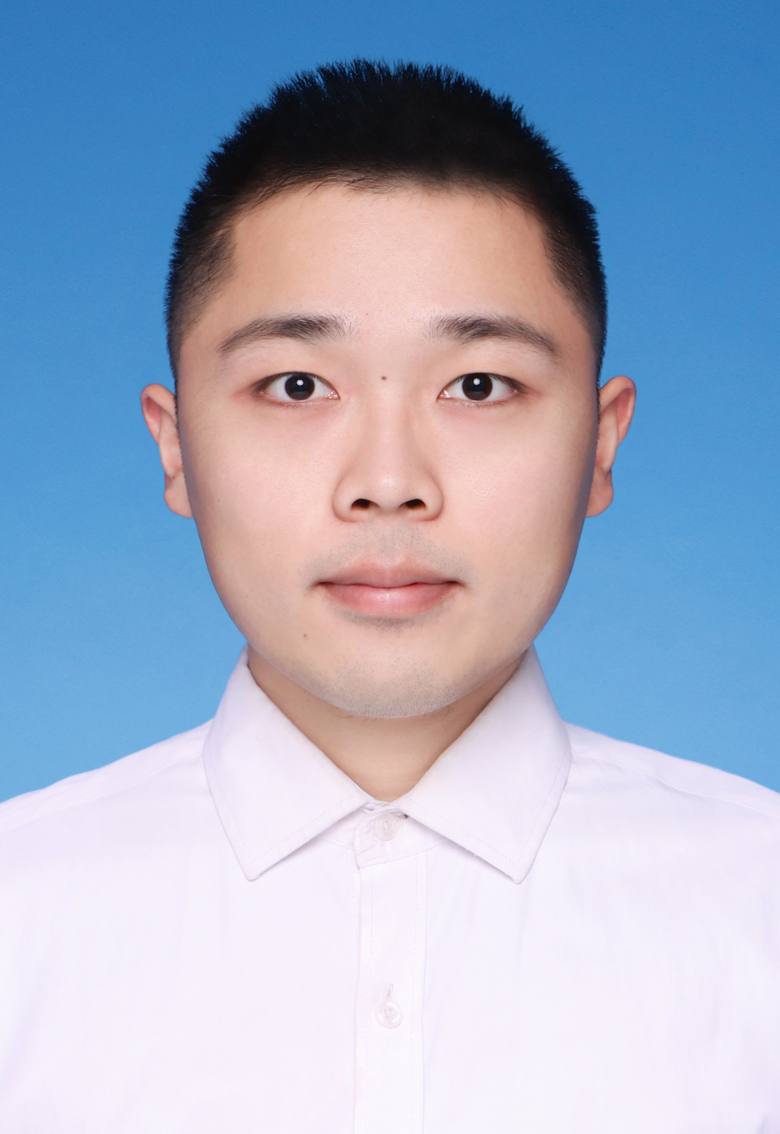
\includegraphics[width=0.50\linewidth,
						height=0.22\paperheight,
						keepaspectratio]{photo.jpg}
						
						\vspace{0.3em}
						{\fontsize{14}{18}\selectfont\bfseries\sffamily 何\quad 亮}
						
						\vspace{0.5em}
						\begin{tcolorbox}[
							colback=structure.fg, colframe=structure.fg,
							arc=4pt, boxrule=0pt,
							top=3pt, bottom=3pt, left=6pt, right=6pt,
							width=0.78\linewidth]
							\centering\color{white}\bfseries\small\sffamily 研究方向
						\end{tcolorbox}
						
						\vspace{4pt}
						\tcbox[on line, arc=4pt, colback=white, colframe=tagborder,
						boxrule=0.8pt, top=1.5pt, bottom=1.5pt, left=5pt, right=5pt,
						fontupper=\footnotesize\bfseries\sffamily\color{structure.fg}]
						{偏微分方程数值方法}\\[3pt]
						\tcbox[on line, arc=4pt, colback=white, colframe=tagborder,
						boxrule=0.8pt, top=1.5pt, bottom=1.5pt, left=5pt, right=5pt,
						fontupper=\footnotesize\bfseries\sffamily\color{structure.fg}]
						{连续体结构拓扑优化}\\[3pt]
						\tcbox[on line, arc=4pt, colback=white, colframe=tagborder,
						boxrule=0.8pt, top=1.5pt, bottom=1.5pt, left=5pt, right=5pt,
						fontupper=\footnotesize\bfseries\sffamily\color{structure.fg}]
						{科学计算软件设计与实现}
					\end{center}
				\end{column}
				
				% ══════════════════════════════════════════
				% 右栏：研究主线 + 研究目标
				% ══════════════════════════════════════════
				\begin{column}{0.62\linewidth}
					\vspace{-1.0em}
					
					% ── 研究主线 ────────────────────────────
					\begin{tcolorbox}[
						colback=structure.fg, colframe=structure.fg,
						arc=4pt, boxrule=0pt,
						top=3pt, bottom=3pt, left=8pt, right=8pt,
						width=\linewidth]
						\centering\color{white}\bfseries\small\sffamily 研究主线
					\end{tcolorbox}
					
					\vspace{3pt}
					{\fontsize{7.5}{10}\selectfont
						围绕基于高阶有限元的变密度拓扑优化开展系统研究，重点关注四个方面：}
					
					\vspace{4pt}
					\begin{tabular}{@{}l@{\hspace{4pt}}l@{}}
						\circnum{01}~%
						\begin{minipage}[c]{2.6cm}
							\begin{tcolorbox}[colback=panelbg!50, colframe=panelbg,
								arc=2pt, boxrule=0.5pt,
								top=2pt, bottom=2pt, left=4pt, right=4pt, nobeforeafter]
								\fontsize{7}{9}\selectfont 高阶有限元拓扑优化方法
							\end{tcolorbox}
						\end{minipage}
						&
						\circnum{03}~%
						\begin{minipage}[c]{2.6cm}
							\begin{tcolorbox}[colback=panelbg!50, colframe=panelbg,
								arc=2pt, boxrule=0.5pt,
								top=2pt, bottom=2pt, left=4pt, right=4pt, nobeforeafter]
								\fontsize{7}{9}\selectfont 胡张混合有限元拓扑优化方法
							\end{tcolorbox}
						\end{minipage}
						\\[6pt]
						\circnum{02}~%
						\begin{minipage}[c]{2.6cm}
							\begin{tcolorbox}[colback=panelbg!50, colframe=panelbg,
								arc=2pt, boxrule=0.5pt,
								top=2pt, bottom=2pt, left=4pt, right=4pt, nobeforeafter]
								\fontsize{7}{9}\selectfont 多分辨率拓扑优化框架
							\end{tcolorbox}
						\end{minipage}
						&
						\circnum{04}~%
						\begin{minipage}[c]{2.6cm}
							\begin{tcolorbox}[colback=panelbg!50, colframe=panelbg,
								arc=2pt, boxrule=0.5pt,
								top=2pt, bottom=2pt, left=4pt, right=4pt, nobeforeafter]
								\fontsize{7}{9}\selectfont SOPTX 软件平台设计与实现
							\end{tcolorbox}
						\end{minipage}
					\end{tabular}
					
					\vspace{6pt}
					% ── 研究目标 ────────────────────────────
					\begin{tcolorbox}[
						colback=structure.fg, colframe=structure.fg,
						arc=4pt, boxrule=0pt,
						top=3pt, bottom=3pt, left=8pt, right=8pt,
						width=\linewidth]
						\centering\color{white}\bfseries\small\sffamily 研究目标
					\end{tcolorbox}
					
					\vspace{4pt}
					{\fontsize{8}{11}\selectfont
						面向复杂结构轻量化设计需求，围绕高精度分析、高效优化求解与软件平台实现，提升连续体结构拓扑优化的理论研究水平与工程应用能力。}
					
				\end{column}
			\end{columns}
		\end{frame}
	}%
	
	% ============================================================
	%  01-2  研究背景与方法设计
	% ============================================================
	\begin{frame}
		\frametitle{研究背景与方法设计}
		
		\vspace{-2em}   % 新增此行
		
		\begin{columns}[t, totalwidth=\linewidth]	
			% ══════════════════════════════════════════════════════
			%  左列：领域关键问题
			% ══════════════════════════════════════════════════════
			\begin{column}{0.48\linewidth}
				\begin{tcolorbox}[
					colback=structure.fg, colframe=structure.fg,
					coltext=white, boxrule=0pt, arc=2pt,
					top=3pt, bottom=3pt, left=6pt, right=6pt,
					]
					\centering\bfseries 领域关键问题
				\end{tcolorbox}
				
				\vspace{0.4em}
				
				\begin{tcolorbox}[
					colback=panelbg, colframe=structure.fg!50,
					boxrule=0.5pt, arc=2pt,
					top=6pt, bottom=6pt, left=6pt, right=6pt,
					]
					{\fontsize{7.5}{11}\selectfont\sffamily
						\textbf{问题 1：物理场分析精度受限}
						\setlength{\itemsep}{2pt}
						\setlength{\parsep}{0pt}
						\setlength{\topsep}{4pt}
						\begin{itemize}
							\item 传统低阶位移元易产生“虚假刚度”，影响位移分析与性能评估的可靠性；
							\item 面向局部应力约束优化时，应力场刻画能力不足，约束评估精度与求解稳定性面临挑战。
						\end{itemize}
						
						\vspace{8pt}
						\textbf{问题 2：高分辨率与计算规模难以兼顾}
						\setlength{\itemsep}{2pt}
						\setlength{\parsep}{0pt}
						\setlength{\topsep}{4pt}
						\begin{itemize}
							\item 单分辨率框架下，设计分辨率的提高伴随分析自由度增长，高精度物理分析与高分辨率结构描述难以同时兼顾。
						\end{itemize}
					}
				\end{tcolorbox}
			\end{column}
			
			\hfill
			
			% ══════════════════════════════════════════════════════
			%  右列：核心方法思路
			% ══════════════════════════════════════════════════════
			\begin{column}{0.48\linewidth}
				\begin{tcolorbox}[
					colback=structure.fg, colframe=structure.fg,
					coltext=white, boxrule=0pt, arc=2pt,
					top=3pt, bottom=3pt, left=6pt, right=6pt,
					]
					\centering\bfseries 核心方法设计
				\end{tcolorbox}
				
				\vspace{0.4em}
				
				\begin{tcolorbox}[
					colback=panelbg, colframe=structure.fg!50,
					boxrule=0.5pt, arc=2pt,
					top=6pt, bottom=6pt, left=6pt, right=6pt,
					]
					{\fontsize{7.5}{11}\selectfont\sffamily
						\textbf{方法 1：高阶离散与混合建模}
						\setlength{\itemsep}{2pt}
						\setlength{\parsep}{0pt}
						\setlength{\topsep}{4pt}
						\begin{itemize}
							\item \textbf{任意次拉格朗日元：}显著削弱虚假刚度，提升位移分析精度；
							\item \textbf{任意次胡张混合有限元：}直接高精度求解应力场，实现大规模局部应力约束的高效稳定求解。
						\end{itemize}
						
						\vspace{8pt}
						\textbf{方法 2：多分辨率拓扑优化框架}
						\setlength{\itemsep}{2pt}
						\setlength{\parsep}{0pt}
						\setlength{\topsep}{4pt}
						\begin{itemize}
							\item 构建分析与设计相解耦的多分辨率框架，在控制计算规模的同时兼顾高精度分析与高分辨率设计。
						\end{itemize}
					}
				\end{tcolorbox}
			\end{column}
			
		\end{columns}
		
	\end{frame}
	
	% ============================================================
	%  01-3  统一软件平台的设计与实现：SOPTX 框架
	% ============================================================
	\begin{frame}
		\frametitle{SOPTX：统一拓扑优化平台的设计与实现}
		
		\vspace{-2em}
		
		\begin{columns}[t, totalwidth=\linewidth]
			
			% ══════════════════════════════════════════════════════
			%  左列：传统实现的关键局限
			% ══════════════════════════════════════════════════════
			\begin{column}{0.48\linewidth}
				\begin{tcolorbox}[
					colback=structure.fg, colframe=structure.fg,
					coltext=white, boxrule=0pt, arc=2pt,
					top=3pt, bottom=3pt, left=6pt, right=6pt,
					]
					\centering\bfseries 传统实现的关键局限
				\end{tcolorbox}
				
				\vspace{-0.2em}
				
				\begin{tcolorbox}[
					colback=panelbg, colframe=structure.fg!50,
					boxrule=0.5pt, arc=2pt,
					top=6pt, bottom=6pt, left=6pt, right=6pt,
					]
					{\fontsize{7.5}{11}\selectfont\sffamily
						\textbf{局限 1：代码极度耦合，扩展困难}
						\setlength{\itemsep}{2pt}
						\setlength{\parsep}{0pt}
						\setlength{\topsep}{4pt}
						\begin{itemize}
							\item 传统程序往往缺乏统一架构，不同算法、离散模型与求解流程之间耦合度高，新方法集成与复用成本较高。
						\end{itemize}
						
						\vspace{3pt}
						\textbf{局限 2：计算效率受硬件条件限制}
						\setlength{\itemsep}{2pt}
						\setlength{\parsep}{0pt}
						\setlength{\topsep}{4pt}
						\begin{itemize}
							\item 传统实现多依赖单一 CPU 串行或浅层并行，面对高分辨率、大规模问题时计算效率受限。
						\end{itemize}
						
						\vspace{3pt}
						\textbf{局限 3：复杂灵敏度推导与实现繁琐}
						\setlength{\itemsep}{2pt}
						\setlength{\parsep}{0pt}
						\setlength{\topsep}{4pt}
						\begin{itemize}
							\item 面对局部应力等复杂约束时，解析灵敏度推导与实现过程繁琐，易出错且维护成本高。
						\end{itemize}
					}
				\end{tcolorbox}
			\end{column}
			
			\hfill
			
			% ══════════════════════════════════════════════════════
			%  右列：SOPTX 框架的核心架构突破
			% ══════════════════════════════════════════════════════
			\begin{column}{0.48\linewidth}
				\begin{tcolorbox}[
					colback=structure.fg, colframe=structure.fg,
					coltext=white, boxrule=0pt, arc=2pt,
					top=3pt, bottom=3pt, left=6pt, right=6pt,
					]
					\centering\bfseries SOPTX 的核心设计
				\end{tcolorbox}
				
				\vspace{-0.2em}
				
				\begin{tcolorbox}[
					colback=panelbg, colframe=structure.fg!50,
					boxrule=0.5pt, arc=2pt,
					top=6pt, bottom=6pt, left=6pt, right=6pt,
					]
					{\fontsize{7.5}{11}\selectfont\sffamily
						\textbf{设计 1：高度模块化架构}
						\setlength{\itemsep}{2pt}
						\setlength{\parsep}{0pt}
						\setlength{\topsep}{4pt}
						\begin{itemize}
							\item 对高阶有限元、胡张混合有限元、多分辨率机制等关键组件进行统一封装，实现算法模块的灵活组合与平滑扩展。
						\end{itemize}
						
						\vspace{3pt}
						\textbf{设计 2：多后端与异构加速机制}
						\setlength{\itemsep}{2pt}
						\setlength{\parsep}{0pt}
						\setlength{\topsep}{4pt}
						\begin{itemize}
							\item 依托 FEALPy 统一张量接口，支持 NumPy、PyTorch、JAX 等后端，实现 CPU/GPU 灵活切换与加速执行。
						\end{itemize}
						
						\vspace{3pt}
						\textbf{设计 3：自动微分驱动的灵敏度实现}
						\setlength{\itemsep}{2pt}
						\setlength{\parsep}{0pt}
						\setlength{\topsep}{4pt}
						\begin{itemize}
							\item 引入自动微分机制，降低复杂灵敏度实现负担，支撑大规模局部应力约束的稳定求解。
						\end{itemize}
					}
				\end{tcolorbox}
			\end{column}
			
		\end{columns}
		
	\end{frame}
	
	% ============================================================
	%  01-4 论文成果
	% ============================================================
	
	\begin{frame}
		\frametitle{论文成果}
		
		% ── 主体：左卡片 + 右卡片 ───────────────────────────────────
		\begin{columns}[T, totalwidth=\linewidth]
			
			% ── 左侧卡片：第一作者论文 ────────────────────────────
			\begin{column}{0.50\linewidth}
				\begin{tcolorbox}[
					colback=white, colframe=structure.fg!50,
					colbacktitle=structure.fg, coltitle=white,
					fonttitle=\fontsize{7.5}{10}\selectfont\bfseries\sffamily,
					title={\circnum{01}\enspace 代表性论文（第一作者）},
					arc=3pt, boxrule=0.5pt,
					toptitle=2pt, bottomtitle=2pt,
					top=7pt, bottom=7pt, left=8pt, right=8pt,
					height=0.60\paperheight, valign=top]
					\setlength{\parskip}{0pt}
					
					{\fontsize{7.5}{12}\selectfont\sffamily\bfseries
						SOPTX: A Modular and Extensible Framework for
						Topology Optimization with Multi-Backend Support\par}
					
					\vspace{-4pt}
					{\color{structure.fg!30}\rule{\linewidth}{0.4pt}}
					\vspace{-8pt}
					
					{\fontsize{7.5}{11}\selectfont\sffamily
						\textbf{发表情况：}\textit{Communications in Computational Physics}，已录用\par
						
						\vspace{2pt}
						\textbf{主要内容：}围绕拓扑优化软件平台的设计与实现，系统研究了模块化架构、%
						面向多后端与异构设备的统一执行机制，以及典型优化模型与算法的集成实现。}
					
				\end{tcolorbox}
			\end{column}
			
			% ── 右侧卡片：两篇合作论文 ────────────────────────────
			\begin{column}{0.47\linewidth}
				\begin{tcolorbox}[
					colback=white, colframe=structure.fg!50,
					colbacktitle=structure.fg, coltitle=white,
					fonttitle=\fontsize{7.5}{10}\selectfont\bfseries\sffamily,
					title={\circnum{02}\enspace 合作研究成果（本人参与）},
					arc=3pt, boxrule=0.5pt,
					toptitle=2pt, bottomtitle=2pt,
					top=7pt, bottom=7pt, left=7pt, right=7pt,
					height=0.60\paperheight, valign=top]
					\setlength{\parskip}{0pt}
					
					% 第一篇
					{\fontsize{7.5}{12}\selectfont\sffamily\bfseries
						Adaptive finite element method for phase field
						fracture models based on recovery error estimates\par}
					
					{\fontsize{7}{10.5}\selectfont\sffamily
						\textbf{发表情况：}\textit{Journal of Computational and Applied Mathematics}, 2026, 472: 116732}
					
					\vspace{-4pt}
					{\color{structure.fg!25}\rule{\linewidth}{0.4pt}}
					\vspace{-8pt}
					
					% 第二篇
					{\fontsize{7.5}{12}\selectfont\sffamily\bfseries
						FEALPy: A Cross-platform Intelligent Numerical
						Simulation Engine\par}
					
					{\fontsize{7}{10.5}\selectfont\sffamily
						\textbf{发表情况：}\textit{Communications in Computational Physics}，已录用}
					
				\end{tcolorbox}
			\end{column}
			
		\end{columns}
		
	\end{frame}
	
	% ============================================================
	%  01-5 软件著作权
	% ============================================================
	
	\begin{frame}
		\frametitle{软件著作权}
		
		% ── 主体：左卡片 + 右卡片 ───────────────────────────────────
		\begin{columns}[T, totalwidth=\linewidth]
			
			% ── 左侧卡片：核心软件成果 ────────────────────────────
			\begin{column}{0.50\linewidth}
				\begin{tcolorbox}[
					colback=white, colframe=structure.fg!50,
					colbacktitle=structure.fg, coltitle=white,
					fonttitle=\fontsize{7.5}{10}\selectfont\bfseries\sffamily,
					title={\circnum{01}\enspace 核心软件成果},
					arc=3pt, boxrule=0.5pt,
					toptitle=2pt, bottomtitle=2pt,
					top=7pt, bottom=7pt, left=8pt, right=8pt,
					height=0.60\paperheight, valign=top]
					\setlength{\parskip}{0pt}
					
					{\fontsize{8}{12}\selectfont\sffamily\bfseries
						结构拓扑优化仿真计算软件\par}
					
					\vspace{-4pt}
					{\color{structure.fg!30}\rule{\linewidth}{0.4pt}}
					\vspace{-8pt}
					
					% 登记信息块
					{\fontsize{7}{10}\selectfont\sffamily\bfseries 登记信息\par}
					\vspace{2pt}
					{\fontsize{7}{10.5}\selectfont\sffamily
						\begin{tabular}{@{}l@{~~}l@{}}
							专利申请号：& 2025SR0887352 \\[1pt]
							专利授权号：& 软著登字第15543550号 \\[1pt]
							本人排名：& 第一完成人 \\
						\end{tabular}\par}
					
					\vspace{2pt}
					{\color{structure.fg!30}\rule{\linewidth}{0.4pt}}
					\vspace{-8pt}
					
					% 成果说明块
					{\fontsize{7}{10}\selectfont\sffamily\bfseries 成果说明\par}
					\vspace{2pt}
					{\fontsize{7}{10.5}\selectfont\sffamily
						面向结构拓扑优化问题的数值求解与仿真分析，开发了结构拓扑优化仿真计算软件，%
						实现了相关算法模块与仿真计算功能。\par}
					
				\end{tcolorbox}
			\end{column}
			
			% ── 右侧卡片：相关软件成果 ────────────────────────────
			\begin{column}{0.47\linewidth}
				\begin{tcolorbox}[
					colback=white, colframe=structure.fg!50,
					colbacktitle=structure.fg, coltitle=white,
					fonttitle=\fontsize{7.5}{10}\selectfont\bfseries\sffamily,
					title={\circnum{02}\enspace 相关软件成果},
					arc=3pt, boxrule=0.5pt,
					toptitle=2pt, bottomtitle=2pt,
					top=7pt, bottom=7pt, left=7pt, right=7pt,
					height=0.60\paperheight, valign=top]
					\setlength{\parskip}{0pt}
					
					{\fontsize{8}{12}\selectfont\sffamily\bfseries
						建筑结构力学仿真计算软件\par}
					
					\vspace{-4pt}
					{\color{structure.fg!25}\rule{\linewidth}{0.4pt}}
					\vspace{-8pt}
					
					% 登记信息块
					{\fontsize{7}{10}\selectfont\sffamily\bfseries 登记信息\par}
					\vspace{2pt}
					{\fontsize{7}{10.5}\selectfont\sffamily
						\begin{tabular}{@{}l@{~~}l@{}}
							专利申请号：& 2024SR0961048 \\[1pt]
							专利授权号：& 软著登字第13364921号 \\[1pt]
							本人排名：& 第三完成人 \\
						\end{tabular}\par}
					
					\vspace{2pt}
					{\color{structure.fg!30}\rule{\linewidth}{0.4pt}}
					\vspace{-8pt}
					
					% 成果说明块
					{\fontsize{7}{10}\selectfont\sffamily\bfseries 成果说明\par}
					\vspace{2pt}
					{\fontsize{7}{10.5}\selectfont\sffamily
						围绕建筑结构力学仿真计算，参与了相关软件开发工作，%
						形成了面向力学分析的软件成果积累。\par}
					
				\end{tcolorbox}
			\end{column}
			
		\end{columns}
		
	\end{frame}
	
	% ============================================================
	%  01-6  参与项目与工程实践
	% ============================================================
	\begin{frame}
		\frametitle{工程应用与核心算法实践}
		
		\vspace{-0.5em}
		
		\begin{columns}[T, totalwidth=\linewidth]
			
			% ── 左侧卡片 ─────────────────────────────────────────────
			\begin{column}{0.50\linewidth}
				\begin{tcolorbox}[
					colback=white, colframe=structure.fg!50,
					colbacktitle=structure.fg, coltitle=white,
					fonttitle=\fontsize{7.5}{10}\selectfont\bfseries\sffamily,
					title={\circnum{01}\enspace 中建智拓计算内核开发},
					arc=3pt, boxrule=0.5pt,
					toptitle=2pt, bottomtitle=2pt,
					top=7pt, bottom=7pt, left=8pt, right=8pt,
					height=0.60\paperheight, valign=top,
					]
					\setlength{\parskip}{0pt}
					
					{\fontsize{8}{12}\selectfont\sffamily\bfseries
						中国建筑第五工程局有限公司合作项目\par}
					
					\vspace{-4pt}
					{\color{structure.fg!30}\rule{\linewidth}{0.4pt}}
					\vspace{-6pt}
					
					{\fontsize{7}{10}\selectfont\sffamily\bfseries 本人角色：主要参与人\par}
					
					\vspace{-4pt}
					{\color{structure.fg!30}\rule{\linewidth}{0.4pt}}
					\vspace{-6pt}
					
					{\fontsize{7}{10}\selectfont\sffamily\bfseries 项目说明\par}
					\vspace{2pt}
					{\fontsize{7}{10.5}\selectfont\sffamily
						面向建筑结构力学分析计算场景，参与中建智拓 C++ 计算内核的设计与实现；\par
						\vspace{4pt}
						围绕跨平台与可扩展结构力学仿真计算需求，开展相关数值计算模块开发、%
						结果验证与文档交付工作。\par}
					
				\end{tcolorbox}
			\end{column}
			
			\hfill
			
			% ── 右侧卡片 ─────────────────────────────────────────────
			\begin{column}{0.47\linewidth}
				\begin{tcolorbox}[
					colback=white, colframe=structure.fg!50,
					colbacktitle=structure.fg, coltitle=white,
					fonttitle=\fontsize{7.5}{10}\selectfont\bfseries\sffamily,
					title={\circnum{02}\enspace FEALPy 核心模块开发},
					arc=3pt, boxrule=0.5pt,
					toptitle=2pt, bottomtitle=2pt,
					top=7pt, bottom=7pt, left=7pt, right=7pt,
					height=0.60\paperheight, valign=top,
					]
					\setlength{\parskip}{0pt}
					
					{\fontsize{8}{12}\selectfont\sffamily\bfseries
						CAX 仿真计算引擎 FEALPy\par}
					
					\vspace{-4pt}
					{\color{structure.fg!25}\rule{\linewidth}{0.4pt}}
					\vspace{-6pt}
					
					{\fontsize{7}{10}\selectfont\sffamily\bfseries 本人角色：主要参与人\par}
					
					\vspace{-4pt}
					{\color{structure.fg!30}\rule{\linewidth}{0.4pt}}
					\vspace{-6pt}
					
					{\fontsize{7}{10}\selectfont\sffamily\bfseries 项目说明\par}
					\vspace{2pt}
					{\fontsize{7}{10.5}\selectfont\sffamily
						参与 FEALPy 仿真计算引擎核心模块开发，负责计算固体力学相关功能实现；\par
						\vspace{4pt}
						围绕线弹性方程、弹塑性方程等问题，开展求解器底层实现与有限元数值模拟功能开发。\par}
					
				\end{tcolorbox}
			\end{column}
			
		\end{columns}
		
	\end{frame}
	
	
	% ============================================================
	\section{片段教学 - 函数极限的夹逼性定理}
	% ============================================================
	
	% ============================================================
	%  02-1  片段教学
	% ============================================================
	
	\begin{frame}
		\frametitle{片段教学}
		
		\vspace{0.6em}
		
		% ── 中部主题区 ──────────────────────────────────────────
		\begin{tcolorbox}[
			colback=structure.fg, colframe=structure.fg,
			arc=6pt, boxrule=0pt,
			top=14pt, bottom=14pt, left=10pt, right=10pt,
			width=\linewidth]
			\centering
			{\fontsize{16}{22}\selectfont\bfseries\sffamily\color{white}
				函数极限的夹逼性定理}\\[6pt]
			{\fontsize{9}{13}\selectfont\sffamily\color{white!80!structure.fg}
				数学分析\ ｜\ 函数极限的性质}
		\end{tcolorbox}
		
		\vspace{1.0em}
		
		% ── 下部目标区 ──────────────────────────────────────────
		\begin{tcolorbox}[
			colback=white, colframe=structure.fg!50,
			colbacktitle=structure.fg, coltitle=white,
			fonttitle=\fontsize{10}{15}\selectfont\bfseries\sffamily,
			title={\enspace 教学目标},
			arc=3pt, boxrule=0.5pt,
			toptitle=0.25pt, bottomtitle=0.25pt,
			top=3pt, bottom=3pt, left=6pt, right=6pt]
			\setlength{\parskip}{0pt}
			{\fontsize{9}{14}\selectfont\sffamily
				\begin{tabular}{@{}c@{\hspace{10pt}}p{0.85\linewidth}@{}}
					\circnum{01} & 理解夹逼性定理的内容及适用条件 \\[10pt]
					\circnum{02} & 能从图像角度直观理解夹逼思想   \\[10pt]
					\circnum{03} & 会用夹逼性定理求简单函数极限   \\
				\end{tabular}
			}
		\end{tcolorbox}
		
	\end{frame}
	
	% ============================================================
	%  02-2  问题引入与思考
	% ============================================================
	
	\begin{frame}
		\frametitle{问题引入与思考}
		
		\vspace{0.3em}
		
		\begin{columns}[T, totalwidth=\linewidth]
			
			% ══════════════════════════════════════════
			% 左列：板块一 现有工具的失效
			% ══════════════════════════════════════════
			\begin{column}{0.48\linewidth}
				\onslide<1->{
					\begin{tcolorbox}[
						colback=white, colframe=structure.fg!50,
						arc=3pt, boxrule=0.5pt,
						top=6pt, bottom=6pt, left=8pt, right=8pt]
						\setlength{\parskip}{0pt}
						{\fontsize{8.5}{13}\selectfont\sffamily
							
							% ── 求解 ──
							\textbf{求解：}探讨函数极限
							$\displaystyle\lim_{x \to 0} x \sin\dfrac{1}{x}$
							
							\par\vspace{3pt}
							\textcolor{structure.fg!60}{\rule{\linewidth}{0.4pt}}
							\par\vspace{3pt}
							
							% ── 分析 ──
							\textbf{分析：}已知 $\lim_{x \to 0} x = 0$，但当 $x \to 0$ 时，
							$\sin\dfrac{1}{x}$ 在 $[-1,1]$ 之间无限振荡，极限不存在。
						
							\par\vspace{3pt}
							\textcolor{structure.fg!60}{\rule{\linewidth}{0.4pt}}
							\par\vspace{3pt}
							
							% ── 困境 ──
							\textbf{困境：}极限的四则运算法则（乘积法则）在此处\textbf{失效}！
					}
					\end{tcolorbox}
				}
			\end{column}
			
			\hfill
			
			% ══════════════════════════════════════════
			% 右列：板块二 知识迁移与启发
			% ══════════════════════════════════════════
			\begin{column}{0.48\linewidth}
				\onslide<2->{
					\begin{tcolorbox}[
						colback=white, colframe=structure.fg!50,
						arc=3pt, boxrule=0.5pt,
						top=6pt, bottom=6pt, left=8pt, right=8pt]
						\setlength{\parskip}{0pt}
						{\fontsize{8.5}{13}\selectfont\sffamily
							
							% ── 回顾 ──
							\textbf{回顾：数列极限的夹逼定理}
							
							\par\vspace{5pt}
							若三个数列 $\{x_n\},\{y_n\},\{z_n\}$ 从某项开始成立
							{\setlength{\abovedisplayskip}{2pt}
								\setlength{\belowdisplayskip}{2pt}
								\[
								x_n \leq y_n \leq z_n,\quad n > N_0,
								\]}
							且 $\lim_{n\to\infty}x_n = \lim_{n\to\infty}z_n = a$，则 $\lim_{n\to\infty}y_n = a$。
							
							\par\vspace{3pt}
							\textcolor{structure.fg!60}{\rule{\linewidth}{0.4pt}}
							\par\vspace{3pt}
							
							% ── 思考 ──
							\textbf{思考：}对于连续的函数，能否借鉴数列极限中
							的放缩思想，通过边界来确定该函数的极限？
						}
					\end{tcolorbox}
				}
			\end{column}
			
		\end{columns}
		
	\end{frame}
	
	% ============================================================
	%  02-3  夹逼性定理
	% ============================================================
	
	\begin{frame}
		\frametitle{夹逼性定理}
		
		\vspace{0.5em}
		
		% ── 定理主体 ────────────────────────────────────────────
		\onslide<1->{
			\begin{tcolorbox}[
				colback=white, colframe=structure.fg!50,
				colbacktitle=structure.fg, coltitle=white,
				fonttitle=\fontsize{10}{15}\selectfont\bfseries\sffamily,
				title={夹逼定理（The Squeeze Theorem）},
				arc=3pt, boxrule=0.5pt,
				toptitle=0.25pt, bottomtitle=0.25pt,
				top=8pt, bottom=8pt, left=12pt, right=12pt]
				{\fontsize{9}{14}\selectfont\sffamily
					若存在 $r>0$，使得当 $0 < |x - x_0| < r$ 时，成立
					{\setlength{\abovedisplayskip}{2pt}
						\setlength{\belowdisplayskip}{2pt}
						\[
						g(x) \leq f(x) \leq h(x),
						\]}
					且 $\lim_{x \to x_0} g(x) = \lim_{x \to x_0} h(x) = A$，%
					则 $\lim_{x \to x_0} f(x) = A$。
				}
			\end{tcolorbox}
		}
		
		\vspace{0.4em}
		% ── 理解要点 ────────────────────────────────────────────
		\begin{tcolorbox}[
			colback=panelbg, colframe=structure.fg!50,
			colbacktitle=structure.fg, coltitle=white,
			fonttitle=\fontsize{10}{15}\selectfont\bfseries\sffamily,
			title={理解要点},
			arc=3pt, boxrule=0.5pt,
			toptitle=0.25pt, bottomtitle=0.25pt,
			top=8pt, bottom=8pt, left=12pt, right=12pt]
			\setlength{\parskip}{0pt}
			{\fontsize{9}{14}\selectfont\sffamily
				\begin{tabular}{@{}c@{\hspace{10pt}}p{0.82\linewidth}@{}}
					\circnum{01} & \textbf{夹在中间：}$f(x)$ 被 $g(x)$ 与 $h(x)$ 从两侧夹住 \\[8pt]
					\circnum{02} & \textbf{去心邻域内成立：}不等式只需在 $x_0$ 的某去心邻域内成立 \\[8pt]
					\circnum{03} & \textbf{两边极限相同：}$g(x)$ 与 $h(x)$ 趋向同一极限值 $A$ \\
				\end{tabular}
			}
		\end{tcolorbox}
		
	\end{frame}
	
	% ============================================================
	%  02-4  图像直观（三帧版）
	% ============================================================
	
	\begin{frame}[fragile]
		\frametitle{图像直观}
		
		\vspace{-2em}
		
		% ── 定理回顾（始终显示）────────────────────────────────────
		\begin{tcolorbox}[
			colback=gray!4, colframe=structure.fg!25,
			colbacktitle=structure.fg!45, coltitle=white,
			fonttitle=\fontsize{8}{12}\selectfont\bfseries\sffamily,
			title={\fontsize{6.5}{10}\selectfont\sffamily\mdseries
				【定理回顾】},
			arc=3pt, boxrule=0.4pt,
			toptitle=0.2pt, bottomtitle=0.2pt,
			top=4pt, bottom=4pt, left=10pt, right=10pt]
			{\fontsize{8}{12}\selectfont\sffamily
				若存在 $r>0$，使得当 $0<|x-x_0|<r$ 时，$g(x)\leq f(x)\leq h(x)$，
				且 $\lim_{x\to x_0}g(x)=\lim_{x\to x_0}h(x)=A$，则
				$\lim_{x\to x_0}f(x)=A$。
			}
		\end{tcolorbox}
		
		\vspace{0.25em}
		
		\centering
		\begin{tikzpicture}
			\begin{axis}[
				width=0.88\linewidth,
				height=0.60\paperheight,
				axis lines=center,
				xlabel={$x$}, ylabel={$y$},
				xlabel style={anchor=north east},
				ylabel style={anchor=south east},
				xmin=-2.0, xmax=5.4,
				ymin=-1.2, ymax=9.5,
				xtick={1.5}, xticklabels={},
				ytick={3.5}, yticklabels={},
				tick style={draw=none},
				clip=false,
				axis on top,
				axis line style={-stealth, thick},
				]
				
				% ══════════════════════════════════════════════════
				%  第 3 帧：夹逼阴影区域（须排在曲线之前以正确叠层）
				% ══════════════════════════════════════════════════
				\only<3->{
					\addplot[
					fill=blue!8, fill opacity=0.5, draw=none,
					domain=-1.5:3.8, samples=120
					]
					{0.55*(x-1.5)^2 + 0.09*(x-1.5)^3 + 3.5}
					\closedcycle;
					\addplot[
					fill=white, fill opacity=1, draw=none,
					domain=-1.5:3.8, samples=120
					]
					{-0.35*(x-1.5)^2 + 0.04*(x-1.5)^3 + 3.5}
					\closedcycle;
				}
				
				% ══════════════════════════════════════════════════
				%  第 1 帧（始终显示）：h(x) 上界（蓝色）
				% ══════════════════════════════════════════════════
				\addplot[domain=-1.5:3.8, samples=120,
				very thick, color=blue!75]
				{0.55*(x-1.5)^2 + 0.09*(x-1.5)^3 + 3.5};
				\node[color=blue!75, font=\small\bfseries, anchor=west]
				at (axis cs:3.85, 7.3) {$y=h(x)$};
				
				% ══════════════════════════════════════════════════
				%  第 2 帧：f(x) 被夹函数（红色）
				% ══════════════════════════════════════════════════
				\only<2->{
					\addplot[domain=-1.5:3.8, samples=120,
					very thick, color=red!75]
					{0.02*(x-1.5)^3 + 3.5};
					\node[color=red!75, font=\small\bfseries, anchor=west]
					at (axis cs:3.85, 3.9) {$y=f(x)$};
				}
				
				% ══════════════════════════════════════════════════
				%  第 1 帧（始终显示）：g(x) 下界（绿色）
				% ══════════════════════════════════════════════════
				\addplot[domain=-1.2:3.8, samples=120,
				very thick, color=green!65!black]
				{-0.35*(x-1.5)^2 + 0.04*(x-1.5)^3 + 3.5};
				\node[color=green!65!black, font=\small\bfseries, anchor=west]
				at (axis cs:3.85, 1.7) {$y=g(x)$};
				
				% ══════════════════════════════════════════════════
				%  第 1 帧（始终显示）：辅助虚线 + 轴标签
				% ══════════════════════════════════════════════════
				\addplot[dashed, gray!70, semithick]
				coordinates {(1.5, 0) (1.5, 3.5)};
				\addplot[dashed, gray!70, semithick]
				coordinates {(0, 3.5) (1.5, 3.5)};
				
				\node[font=\small\bfseries, below] at (axis cs:1.5, 0) {$x_0$};
				\node[font=\small\bfseries, left]  at (axis cs:0, 3.5) {$A$};
				
				% ══════════════════════════════════════════════════
				%  汇聚点
				% ══════════════════════════════════════════════════
				%  第 1 帧：蓝、绿色点
				\addplot[only marks, mark=*, mark size=3.0pt, color=blue!75]
				coordinates {(1.5, 3.5)};
				\addplot[only marks, mark=*, mark size=3.0pt, color=green!65!black]
				coordinates {(1.5, 3.5)};
				%  第 2 帧起：加红色点
				\only<2->{
					\addplot[only marks, mark=*, mark size=3.0pt, color=red!75]
					coordinates {(1.5, 3.5)};
				}
				%  第 3 帧：白边衬底
				\only<3->{
					\addplot[only marks, mark=o, mark size=3.8pt,
					mark options={color=white, line width=1.2pt}]
					coordinates {(1.5, 3.5)};
				}
				
				% ══════════════════════════════════════════════════
				%  第 3 帧："挤压"箭头标注
				% ══════════════════════════════════════════════════
				\only<3->{
					\draw[-stealth, gray!60, thin]
					(axis cs:0.3, 6.2) -- (axis cs:1.1, 4.2);
					\node[gray!70, font=\scriptsize, anchor=east]
					at (axis cs:0.25, 6.35) {$h(x_0)=A$};
					
					\draw[-stealth, gray!60, thin]
					(axis cs:0.3, 0.8) -- (axis cs:1.1, 2.8);
					\node[gray!70, font=\scriptsize, anchor=east]
					at (axis cs:0.25, 0.65) {$g(x_0)=A$};
				}
				
			\end{axis}
		\end{tikzpicture}
		
	\end{frame}
	
	% ============================================================
	%  02-5  夹逼性定理的证明
	% ============================================================
	
	\begin{frame}
		\frametitle{夹逼性定理的证明}
		
		\vspace{-0.5em}
		
		\begin{tcolorbox}[
			colback=white, colframe=structure.fg!50,
			colbacktitle=structure.fg, coltitle=white,
			fonttitle=\fontsize{10}{15}\selectfont\bfseries\sffamily,
			title={证明思路：基于 $\varepsilon-\delta$ 语言},
			arc=3pt, boxrule=0.5pt,
			toptitle=0.25pt, bottomtitle=0.25pt,
			top=8pt, bottom=8pt, left=12pt, right=12pt]
			{\fontsize{8.5}{12}\selectfont\sffamily
				
				\textbf{分析：}证 $\lim_{x \to x_0} f(x) = A \iff \forall \varepsilon > 0, \exists \delta > 0, 0 < |x - x_0| < \delta \implies |f(x) - A| < \varepsilon$。
				
				\only<2->{
					\vspace{-2pt}
					\textcolor{structure.fg!60}{\rule{\linewidth}{0.4pt}}
					\vspace{-8pt}
					
					\textbf{证明：}对 $\forall \varepsilon > 0$：
					\begin{itemize}
						\setlength{\itemsep}{4pt}
						\item $\lim_{x \to x_0} g(x) = A \implies \exists \delta_1 > 0$, 当 $0 < |x - x_0| < \delta_1$ 时, $A - \varepsilon < g(x) < A + \varepsilon$;
						\item $\lim_{x \to x_0} h(x) = A \implies \exists \delta_2 > 0$, 当 $0 < |x - x_0| < \delta_2$ 时, $A - \varepsilon < h(x) < A + \varepsilon$。
					\end{itemize}
					
					\vspace{6pt}
					取 $\delta = \min\{\delta_1, \delta_2, r\}$。当 $0 < |x - x_0| < \delta$ 时，由已知 $g(x) \leq f(x) \leq h(x)$ 有：
					{\setlength{\abovedisplayskip}{6pt}
						\setlength{\belowdisplayskip}{6pt}
						\[
						A - \varepsilon < g(x) \leq f(x) \leq h(x) < A + \varepsilon
						\]}
					即 $A - \varepsilon < f(x) < A + \varepsilon \implies |f(x) - A| < \varepsilon$。
					
					\vspace{4pt}
					综上可知，$\lim_{x \to x_0} f(x) = A$。 \hfill $\square$
				}
			}
		\end{tcolorbox}
		
	\end{frame}
	
	% ============================================================
	%  02-6  典型例题（两帧版）
	% ============================================================
	
	\begin{frame}
		\frametitle{典型例题}
		
		\vspace{-0.5em}
		
		\begin{tcolorbox}[
			colback=white, colframe=structure.fg!50,
			colbacktitle=structure.fg, coltitle=white,
			fonttitle=\fontsize{10}{15}\selectfont\bfseries\sffamily,
			title={例题演练},
			arc=3pt, boxrule=0.5pt,
			toptitle=0.25pt, bottomtitle=0.25pt,
			top=10pt, bottom=10pt, left=12pt, right=12pt]
			{\fontsize{9}{13}\selectfont\sffamily
				
				求函数极限 $\displaystyle \lim_{x \to 0} x \sin\tfrac{1}{x}$
				
				\only<2->{
					\vspace{-2pt}
					\textcolor{structure.fg!60}{\rule{\linewidth}{0.4pt}}
					\vspace{-8pt}
					
					{\fontsize{8.5}{12}\selectfont
						\textbf{分析：} 利用 $\sin\frac{1}{x}$ 的有界性进行"放缩"，构造夹逼区间。
						
						\vspace{6pt}
						
						\textbf{解：} $\because |\sin\tfrac{1}{x}| \leq 1$, 对 $\forall x \neq 0$，成立：
						{\setlength{\abovedisplayskip}{6pt}
							\setlength{\belowdisplayskip}{6pt}
							\[
							-|x| \leq x \sin\tfrac{1}{x} \leq |x|
							\]}
						
						\vspace{2pt}
						令 $g(x) = -|x|$, $h(x) = |x|$。由已知极限有：
						{\setlength{\abovedisplayskip}{4pt}
							\setlength{\belowdisplayskip}{4pt}
							\[
							\lim_{x \to 0} g(x) = 0, \quad \lim_{x \to 0} h(x) = 0
							\]}
						
						\vspace{2pt}
						根据\textbf{夹逼性定理}可知：
						{\setlength{\abovedisplayskip}{6pt}
							\setlength{\belowdisplayskip}{6pt}
							\[
							\lim_{x \to 0} x \sin\tfrac{1}{x} = 0 \quad \square
							\]}
					}
				}
			}
		\end{tcolorbox}
		
	\end{frame}
	
	% ============================================================
	%  结束页
	% ============================================================
	\begin{frame}[plain]
		\vspace{1.2cm}
		\begin{center}
			{\fontsize{24}{30}\selectfont\bfseries\sffamily\color{structure.fg} 汇报结束}
			
			\vspace{0.9cm}
			\begin{tcolorbox}[
				colback=panelbg, colframe=structure.fg!45,
				arc=4pt, boxrule=0.6pt,
				top=8pt, bottom=8pt, left=14pt, right=14pt,
				width=0.68\linewidth]
				\centering
				{\fontsize{12}{18}\selectfont\bfseries\sffamily 感谢各位老师聆听}\\[4pt]
				{\fontsize{10}{15}\selectfont\sffamily 恳请批评指正}
			\end{tcolorbox}
			
			\vspace{0.8cm}
			{\fontsize{8}{12}\selectfont\sffamily\color{black!65}
				科研汇报：基于高阶有限元的变密度拓扑优化\\[4pt]
				片段教学：函数极限的夹逼性定理}
		\end{center}
	\end{frame}
	
	
	
\end{document}